\chapter{Implementación}

La implementación del software se ha dividido en hitos. Estos han sido definidos en GitHub
y cada uno de ellos contiene un grupo de \textit{issues} que se corresponden con las distintas
mejoras que se han ido incorporando al software a lo largo de su desarrollo.

Cada milestone representa un bloque de trabajo con un objetivo definido, lo que permite seguir
un enfoque ágil, enfocado en construir progresivamente un prototipo sólido en lugar de intentar
desarrollar todo el sistema de una vez. 

\section{Milestone 1: Elección del lenguaje de programación}
En este primer hito se decidió el lenguaje de programación a utilizar para el desarrollo del software,
siendo Python la opción elegida. Esta elección se justificó y documentó debidamente en el
\hyperref[sec:lenguaje-programación]{anterior capítulo}.

\section{Milestone 2: Modelo del problema}
Este hito se centra en dos tareas principales: la configuración de las herramientas necesarias para
el desarrollo guiado por pruebas, y la definición del modelo del dominio siguiendo el enfoque 
\textit{Domain-Driven Design} (DDD).

\subsection{Configuración del entorno de desarrollo}
En el capítulo anterior se seleccionaron las herramientas que se emplearían para 
\hyperref[sec:gestor-dependencias]{gestionar las dependencias y el entorno} y 
\hyperref[sec:herramienta-testeo]{realizar pruebas}. En este hito se procedió a su instalación y 
configuración.

\subsubsection{Poetry}
Se ha usado \textit{Poetry} para gestionar las dependencias y el entorno virtual del proyecto.

Al inicializar el gestor, se genera automáticamente un archivo \texttt{pyproject.toml} en la raíz del
repositorio, que contiene la información básica del proyecto y servirá como punto central
para la gestión de dependencias.

\subsubsection{Pytest}
La herramienta seleccionada para las pruebas unitarias ha sido \texttt{pytest}.
La elección de esta herramienta ya fue justificada en el capítulo anterior.

Se ha añadido \texttt{pytest} como dependencia, lo que significa que se instalará únicamente
para el entorno de desarrollo y no se considera una dependencia necesaria para la ejecución del 
prototipo en producción. De esta manera se mantiene una separación clara entre las librerías 
empleadas para programar y probar el software, y aquellas que serán estrictamente necesarias para 
su despliegue.

Al instalar dependencias mediante Poetry, junto al archivo \texttt{pyproject.toml} se genera 
automáticamente el archivo \texttt{poetry.lock}. El primero declara qué dependencias se requieren y 
en qué rango de versiones son aceptables; en cambio, el archivo \texttt{poetry.lock} registra la 
versión exacta de esas dependencias en el momento de la instalación. Gracias a este mecanismo se 
garantiza la reproducibilidad del entorno, ya que cualquier persona que clone el repositorio e 
instale las dependencias obtendrá exactamente las mismas versiones usadas en el desarrollo 
original.

\subsection{Modelo del dominio}
El modelado del dominio se ha realizado siguiendo el enfoque \textit{Domain-Driven Design} (DDD)
propuesto por Eric Evans \cite{evansDDD}. Este método de diseño de software se centra en que
el sistema refleje fielmente la realidad del dominio que se está modelando, evitando que los 
aspectos técnicos o de implementación condicionen la representación del problema.

Uno de los principios fundamentales de DDD es la creación de un \textit{lenguaje ubicuo}, introducido
por Evans en el capítulo 2 de su obra \cite{evansDDD}. Esto consiste en definir términos y conceptos 
específicos del dominio para que los conceptos empleados en el código coincidan con los del propio 
dominio. De este modo se facilita la comunicación entre el análisis y la implementación. En este 
proyecto se ha definido el siguiente lenguaje ubicuo:

\begin{itemize}
    \item \textbf{Escudo}: Entendemos como escudo a la representación gráfica de un conjunto de
    elementos heráldicos que identifican a una persona, entidad o institución.
    \item \textbf{Blasón}: Descripción textual del escudo.
    \item \textbf{Portador}: Persona, entidad o institución a la que pertenece el escudo.
    \item \textbf{Campo}: Superficie del escudo donde se disponen los elementos heráldicos.
    \item \textbf{Boca}: Forma exterior del escudo, es decir, su contorno.
    \item \textbf{Partición}: Cada una de las divisiones del campo del escudo. 
    \item \textbf{Esmalte}: Color o metal con el que se pinta un elemento heráldico.
    \item \textbf{Pieza heráldica}: Son elementos de distinto esmalte al del campo que suelen tocar
    los bordes del escudo.
    \item \textbf{Figura o mueble}: Son todo aquello que se encuentra dentro del campo del escudo y
    no resulta ser una pieza heráldica.
    \item \textbf{Adorno exterior}: Son todos aquellos elementos que no se encuentran dentro del campo
    del escudo.
\end{itemize}

\begin{figure}[H]
    \centering
    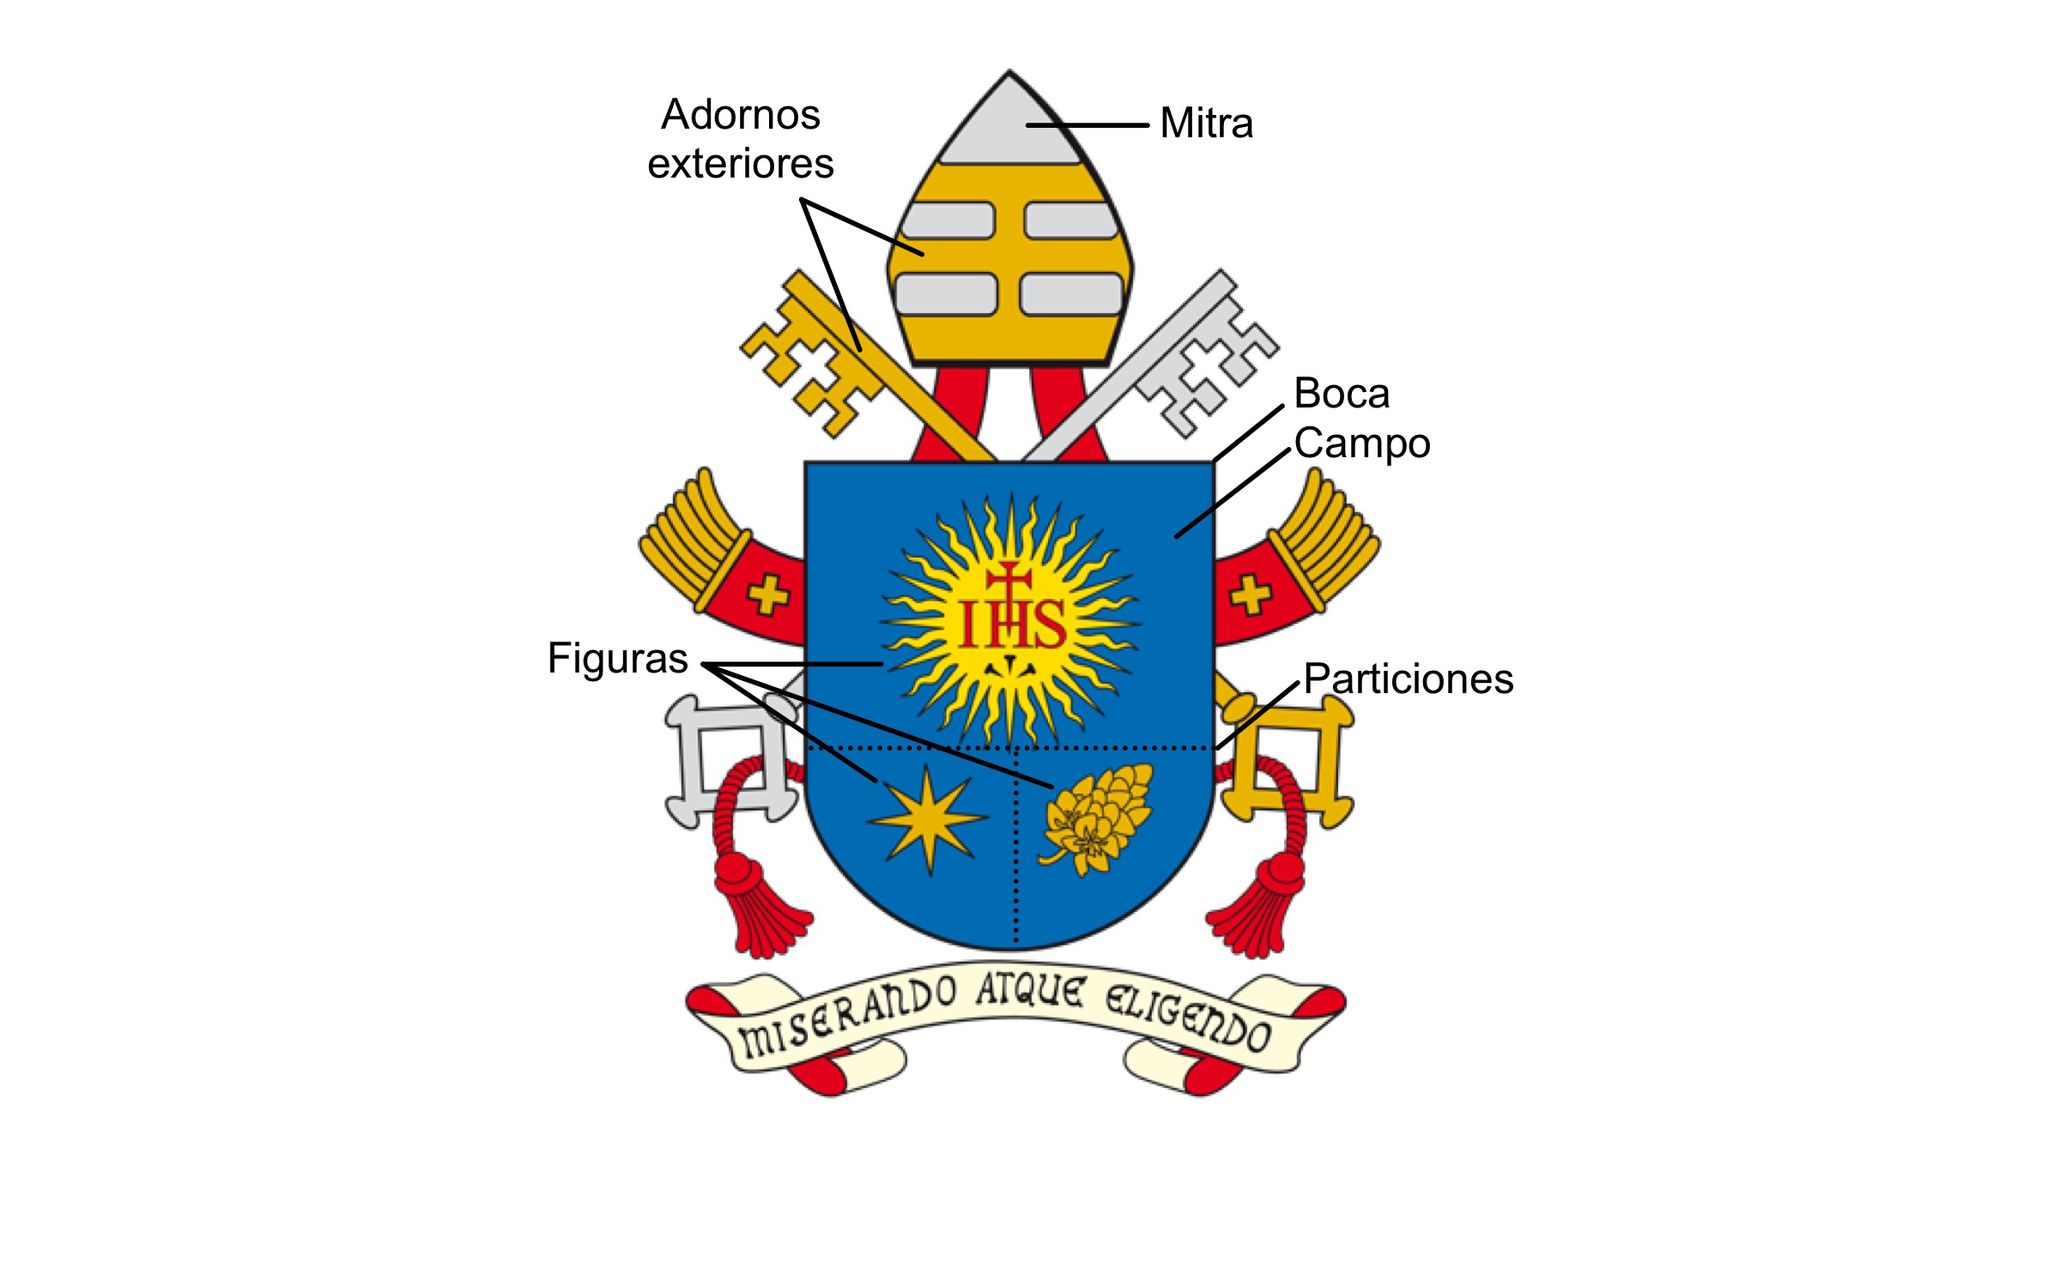
\includegraphics[width=1\textwidth]{figuras/escudo-papa-francisco.png}
    \caption{Partes del escudo de armas del papa Francisco \cite{wikiEscudo}.}
    \label{fig:partes-escudo}
\end{figure}

Las definiciones empleadas en este lenguaje ubicuo se han extraído del 
\textit{Manual de heráldica: la ciencia del blasón} \cite{delgadoHeraldica}.

En esta primera iteración se ha decidido limitar el modelo a una parte reducida del lenguaje ubicuo. 
Concretamente, se trabajará con el \textbf{Escudo} como composición de otros elementos, incorporando 
inicialmente el \textbf{Campo} y el \textbf{Esmalte}, que constituyen la base mínima necesaria para 
definir un prototipo funcional. 

Otros elementos como la \textbf{Boca}, el \textbf{Portador}, las \textbf{Particiones}, las 
\textbf{Piezas heráldicas}, las \textbf{Figuras} o los \textbf{Adornos exteriores} se han recogido 
en el lenguaje ubicuo, pero quedan fuera del alcance de esta iteración y se abordarán en futuras 
extensiones del modelo.

\subsection{Desarrollo dirigido por pruebas (TDD)}

El modelo inicial del dominio se ha implementado siguiendo la metodología de 
\textit{Test-Driven Development} (TDD) \cite{beckTDD}. Esto significa que antes de escribir 
el código se definieron las pruebas que debía superar, y después se implementó lo mínimo necesario 
para que pasaran.

En esta primera iteración se definieron pruebas unitarias para los elementos básicos 
del modelo: \texttt{Esmalte}, \texttt{Campo} y \texttt{Escudo}. Dichas pruebas validan:

\begin{itemize}
    \item Que un \texttt{Escudo} válido puede crearse a partir de un \texttt{Campo} 
    con un \texttt{Esmalte} permitido.
    \item Que los intentos de producir un \texttt{Esmalte} con valores no reconocidos producen 
    una excepción.
    \item Que no es posible instanciar un \texttt{Campo} sin un \texttt{Esmalte} válido.
\end{itemize}

Al principio estas pruebas no pasan, ya que no existe ninguna implementación. A continuación se
escribe el código mínimo necesario para que todas las pruebas definidas pasen correctamente. Esto
se repetirá cada vez que se añada una nueva funcionalidad al modelo.

Como resultado surgieron las clases \texttt{Esmalte}, \texttt{Campo} y \texttt{Escudo}, que constituyen 
la base mínima del dominio:

\begin{itemize}
    \item \texttt{Esmalte}: representa los colores y metales permitidos en heráldica. 
    Comprueba que el valor introducido sea válido y lo normaliza.
    \item \texttt{Campo}: representa la superficie del escudo. Solo puede generarse 
    si se le proporciona un \texttt{Esmalte} válido.
    \item \texttt{Escudo}: actúa como elemento principal y se compone de un \texttt{Campo}.
\end{itemize}

\section{Milestone 3: Identificación y filtrado por esmalte}

En este milestone se introduce la primera lógica de negocio, que consiste en filtrar los escudos
por el esmalte del campo. Esto facilita la identificación de escudos de \hyperref[sec:hu1]{HU1} y 
la clasificación y el filtrado de escudos de \hyperref[sec:hu2]{HU2}.

Para ello, es necesario implementar un catálogo mínimo de ejemplo para poder realizar la consulta.

Los criterios de aceptación son sencillos: (1) dado un esmalte válido, la consulta devuelve 
únicamente escudos con ese campo; (2) sin criterio, se devuelve el catálogo completo; y 
(3) con un criterio erróneo, la respuesta es una lista vacía.

\subsection{Adición de un catálogo mínimo}

En este punto no había ningún escudo cargado y, por tanto, no había nada que filtrar. Antes 
de implementar la búsqueda por esmalte del campo, lo razonable era añadir al sistema un catálogo 
base sobre el que poder trabajar y comprobar el comportamiento.

Para este hito opté por un catálogo mínimo y en memoria, dentro del propio paquete. 
Cada entrada se modela como una pequeña ficha con el nombre del escudo y el esmalte.
El campo se guarda como un Esmalte, de modo que queda validado y normalizado desde
el minuto uno y se evitan incoherencias.

Se han añadido a este catálogo siete escudos, uno para cada esmalte canónico, con la finalidad de
poder probar la búsqueda de cualquier esmalte. La decisión de mantener el catálogo en memoria
simplifica la implementación inicial y permite centrarse en la funcionalidad de filtrado sin
introducir complejidades adicionales que se tratarán en futuros hitos, como la implementación
de una base de datos.

Siguiendo TDD, primero escribí unas pruebas muy básicas: que el catálogo no esté vacío y que el 
campo de cada ficha sea un Esmalte. Con esas pruebas en rojo implementé lo mínimo para ponerlas en
verde: un catálogo pequeño en memoria y la función listar(). Con eso ya está lista la base para el
siguiente paso: filtrar la búsqueda por el esmalte del campo.